%% LyX 2.3.1-1 created this file.  For more info, see http://www.lyx.org/.
%% Do not edit unless you really know what you are doing.
\documentclass[10pt,letterpaper,conference]{ieeeconf}
\usepackage[latin9]{inputenc}
\setcounter{secnumdepth}{3}
\setcounter{tocdepth}{3}
\usepackage{color}
\usepackage{float}
\usepackage{calc}
\usepackage{units}
\usepackage{textcomp}
\usepackage{amsmath}
\usepackage{graphicx}
\usepackage[unicode=true,
 bookmarks=true,bookmarksnumbered=false,bookmarksopen=false,
 breaklinks=false,pdfborder={0 0 0},pdfborderstyle={},backref=false,colorlinks=true]
 {hyperref}
\hypersetup{pdftitle={Gaussian Process Based Model-less Control with Q-Learning},
 pdfauthor={Jan Hauser and Daniel Pachner and Vladim�r Havlena},
 pdfkeywords={Gaussian process, Q-Learning, Model-less Controll, Machine Learning}}

\makeatletter

%%%%%%%%%%%%%%%%%%%%%%%%%%%%%% LyX specific LaTeX commands.
\pdfpageheight\paperheight
\pdfpagewidth\paperwidth

\newcommand{\lyxmathsym}[1]{\ifmmode\begingroup\def\b@ld{bold}
  \text{\ifx\math@version\b@ld\bfseries\fi#1}\endgroup\else#1\fi}

\floatstyle{ruled}
\newfloat{algorithm}{tbp}{loa}
\providecommand{\algorithmname}{Algorithm}
\floatname{algorithm}{\protect\algorithmname}

%%%%%%%%%%%%%%%%%%%%%%%%%%%%%% User specified LaTeX commands.
%%%%%%%%%%%%%%%%%%%%%%%%%%%%%%%%%%%%%%%%%%%%%%%%%%%%%%%%%%%%%%%%%%%%%%%%%%%%%%%%
%2345678901234567890123456789012345678901234567890123456789012345678901234567890
%        1         2         3         4         5         6         7         8

% Comment this line out if you need a4paper

%\documentclass[a4paper, 10pt, conference]{ieeeconf}      % Use this line for a4 paper

\IEEEoverridecommandlockouts                              % This command is only needed if 
                                                          % you want to use the \thanks command

\overrideIEEEmargins                                      % Needed to meet printer requirements.

%In case you encounter the following error:
%Error 1010 The PDF file may be corrupt (unable to open PDF file) OR
%Error 1000 An error occurred while parsing a contents stream. Unable to analyze the PDF file.
%This is a known problem with pdfLaTeX conversion filter. The file cannot be opened with acrobat reader
%Please use one of the alternatives below to circumvent this error by uncommenting one or the other
%\pdfobjcompresslevel=0
%\pdfminorversion=4

% See the \addtolength command later in the file to balance the column lengths
% on the last page of the document

% The following packages can be found on http:\\www.ctan.org
%\usepackage{graphics} % for pdf, bitmapped graphics files
%\usepackage{epsfig} % for postscript graphics files
%\usepackage{mathptmx} % assumes new font selection scheme installed
%\usepackage{times} % assumes new font selection scheme installed
%\usepackage{amsmath} % assumes amsmath package installed
\usepackage{amssymb}  % assumes amsmath package installed

\title{\LARGE \bf
 Gaussian Process Based Model-less Control with Q-Learning*
}


\author{Jan Hauser$^{1}$, Daniel Pachner$^{2}$ and Vladim�r Havlena$^{1}$% <-this % stops a space
\thanks{*This work has been supported by the project 18-26278S sponsored by Grant Agency of the Czech Republic.}% <-this % stops a space
\thanks{$^{1}$Jan Hauser and Vladim�r Havlena are with Department of Control Engineering, 
Faculty of Electrical Engineering of Czech Technical University in Prague, Technicka 2, 166 27 Praha 6, Czech Republic.
Email: {\tt\small \{hauseja3,havlena\}@fel.cvut.cz}}%
\thanks{$^{2}$Daniel Pachner is with Honeywell HBT Architecture $\&$ Innovation Team, 
V Parku 2326/18, 148 00 Prague, Czech Republic 
Email: {\tt\small daniel.pachner@honeywell.com}}%
}

\makeatother

\begin{document}
\maketitle \thispagestyle{empty} \pagestyle{empty}
\begin{abstract}
The aim of this paper is to demonstrate how Machine Learning (ML)
based on Gaussian Process Regression (GPR) can be used as a practical
control design technique. An optimized control law for a nonlinear
process is found directly by training the algorithm on noisy data
collected from the process when controlled by a sub-optimal controller.
A simplified nonlinear Fan Coil Unit (FCU) model is used as an example
for which the fan speed control is designed using the off-policy Q-Learning
algorithm. Additionally, the algorithm properties are discussed, i.e.
learning process robustness, GP kernel functions choice. The simulation
results are compared to a simple PI, designed based on a linearized
model.
\end{abstract}

\section{INTRODUCTION}

Model-less control techniques assume that no mathematical model of
the controlled process is available and the controller is designed
from the measurement data. One such approach would collect the data
in advance during some time window to use it offline for a controller
design. A different approach would attempt to use the data in the
real time to improve the control continuously. In this article the
former offline approach is considered, i.e. the situation when some
sub-optimal controller was already in use and the data were collected
and can be used to optimize or improve that controller. Many existing
control design techniques first create a model from data to use it
for a control design method afterwards, which makes sense if some
reliable modeling information, e.g. model structure, is available.
A different approach, used in this paper, is the controller designed
directly from the data, without any process model. This approach can
have some advantages especially if little or nothing is known about
the process or if the process is nonlinear and no analytical control
design method is available.

The Q-Learning is an off-policy machine learning (ML) iterative algorithm
\cite{ecc19ref:Sutton_Reinforcement_Learning}, which approximates
certain function satisfying the Bellman equation. This Q function
then defines a controller. Q-Learning was developed for Markov Decision
Process (MDP) with finite number of states and later generalized to
continuous state spaces \cite{ecc19ref:Hasselt_Reinforcement_learning_in_continuous_action_spaces,ecc19ref:Gaskett_Q_Learning_IC}.
If the analytical form of the Q function is unknown in continuous
state spaces, it may be represented by an universal function approximating
method such as Neural Network or Gaussian Process Regression (GPR).

GPR is a non-parametric regression technique \cite{ecc19ref:Rasmussen_Gaussian_Processes}
which is able to approximate any continuous target function uniformly.
Unfortunately, the runtime computational requirement is $\mathcal{O}(n^{3})$
and the memory requirement is $\mathcal{O}(n^{2})$ for $n$ data
points. Various sparse GPR techniques were developed to overcome this
computational complexity \cite{ecc19ref:Bijl_Online_Sparse_Gaussian,ecc19ref:Candela_A_unifying_view,ecc19ref:Huber_Recursive_GP}.
One of the conventional GPR sparse method is to use a set of size
$m$ induction input points, which reduce the computational complexity
to $\mathcal{O}(nm^{2})$ (runtime) and $\mathcal{O}(nm)$ (memory).
These induction points reduce the whole dataset into a smaller number
of representing data points, which are distributed across the data
space to preserve as much information as possible. GP uses various
covariance (kernel) functions \cite{ecc19ref:Williams_Prediction_with_Gaussian_processes}
to define the data covariance matrices. The choice of the kernel can
have significant impact on the accuracy of the regression model.

The contribution of this paper is the practical and efficient combination
of Q-Learning and GPR resulting in unbiased estimate of the Q function.
ML algorithms are normally supposed to process a large dataset (of
size $\sim10^{5}$ and more) to yield sufficiently accurate results.
Often the training data are simulated by a model and the statistical
properties of the algorithm are thus less important. Here a smaller
dataset from a process affected by unmeasured disturbances is targeted
(of a size $\sim10^{3}$). This requires the information in the data
to be used efficiently. 

A simple Fan Coil Unit (FCU) model approximation is used to demonstrate
the approach. FCU is a nonlinear system widely used for both air heating
and cooling in buildings. A linear control design cannot achieve optimal
FCU control in terms of energy consumption and user comfort \cite{ecc19ref:Arguello_Serrano_Nonlinear_HVAC}.
FCU model used here is highly simplified to make the result easier
to interpret. It is supposed that ML will be able to optimize a real
FCU control based on several days data.

For reader's understanding, some essential theory is briefly introduced.
In Section \ref{sec:gp}, the GPR algorithm is explained. Section
\ref{sec:Q-Learning} describes the Q-Learning mechanism and how it
connects to GPR. In Section \ref{sec:Fan-Coil-Unit}, a reduced FCU
model is explained. Next Section \ref{sec:RESULTS} presents the results
of these techniques and Section \ref{sec:CONCLUSIONS} concludes and
proposes a future work. 

\section{GAUSSIAN PROCESS\label{sec:gp}}

In this section, GPR method is briefly described. The GPR technique
is then used with Q-Learning algorithm in next section.

\subsection{Gaussian Process Regression}

GPR is a supervised learning regression model, which can be also described
as a distribution over functions \cite{ecc19ref:Rasmussen_Gaussian_Processes}.
It is the function value estimator for an unknown function $f(\mathbf{x})$
considering any dataset $(\mathbf{X},\mathbf{y})$, which can be written
as 

\[
f(\mathbf{x})\sim\mathcal{GP}\left(m(\mathbf{x}),\kappa(\mathbf{x},\mathbf{x}')\right),
\]

\noindent where mean $m(\mathbf{x})$ and covariance function $\kappa(\mathbf{x},\mathbf{x}'$)
are given a priori up to some hyperparameters and are defined as

\begin{eqnarray*}
m(\mathbf{x)} & = & \mathbb{E}\left[f(\mathbf{x})\right],\\
\kappa(\mathbf{x},\mathbf{x}') & = & \mathbb{E}\left[\left(f(\mathbf{x})-m(\mathbf{x})\right)\left(f(\mathbf{x}')-m(\mathbf{x}')\right)^{\top}\right],
\end{eqnarray*}

\noindent where $\mathbb{E}$ is the expectation, $\mathbf{x}$ and
$\mathbf{x}'$ are a pair of vectors in the data space. A dataset
is a number of such vectors $\mathbf{X}=\left\{ \mathbf{x}_{1},\mathbf{x}_{2},\ldots,\mathbf{x}_{n}\right\} $.
In this article $f(\mathbf{x})\in\mathbb{R}.$

Assume the finite training set $\mathbf{X}$ and the finite testing
set $\mathbf{X}_{p}$, then GPR can predict $z_{j}=f(\mathbf{x}_{p_{j}}^{\mathrm{}})$,
where $\mathbf{x}_{p_{j}}^{\mathrm{}}\in\mathbf{X}_{p}$, by using
data $\mathbf{x}_{i}\in\mathbf{X}$ and their function values $f(\mathbf{x}_{i})$.
The function values $f(\mathbf{X})$ themselves do not need to be
accessible but rather their noisy measurements $y_{i}=f(\mathbf{x}_{i})+\varepsilon_{i}$,
where $\varepsilon_{i}$ is independent identically distributed (i.i.d)
Gaussian noise with variance $\sigma_{n}^{2}$. The prior covariance
of the noisy values is defined as 

\begin{equation}
\mathrm{cov}(\mathbf{y})=\kappa(\mathbf{X},\mathbf{X})+\sigma_{n}^{2}\mathbf{I}.\label{eq:covariance-noisy-measurements}
\end{equation}

Then the prior joint probability distribution function (p.d.f) can
be defined for training and testing sets values as 

\begin{multline*}
\left[\begin{array}{c}
\mathbf{y}\\
\mathbf{z}
\end{array}\right]\sim\left[\begin{array}{c}
f(\mathbf{X})+\boldsymbol{\varepsilon}\\
f(\mathbf{X}_{p})
\end{array}\right]\sim\\
\mathcal{N}\left(\left[\begin{array}{c}
m(\mathbf{X})\\
m(\mathbf{X}_{p})
\end{array}\right],\left[\begin{array}{cc}
\kappa(\mathbf{X},\mathbf{X})+\sigma_{n}^{2}\mathbf{I} & \kappa(\mathbf{X},\mathbf{X}_{p})\\
\kappa(\mathbf{X}_{p},\mathbf{X}) & \kappa(\mathbf{X}_{p},\mathbf{X}_{p})
\end{array}\right]\right)=\\
\mathcal{N}\left(\left[\begin{array}{c}
\mathbf{m}\\
\mathbf{m}_{z}
\end{array}\right],\left[\begin{array}{cc}
\mathbf{K}_{ff}+\sigma_{n}^{2}\mathbf{I} & \mathbf{K}_{fz}\\
\mathbf{K}_{zf} & \mathbf{K}_{zz}
\end{array}\right]\right),
\end{multline*}

\noindent where $\mathcal{N}$ is normal distribution defined by
mean and covariance, $\mathbf{K}_{fz}$ is a $n\times n_{p}$ matrix
of the covariances of all pairs of training and testing datasets,
and $\mathbf{K}_{ff}$, $\mathbf{K}_{zz}$, $\mathbf{K}_{zf}$ analogously.
Let's also use a notation $\mathbf{K}_{yy}=\mathbf{K}_{ff}+\sigma_{n}^{2}\mathbf{I}$
for covariance of noisy measurements $\mathbf{y}$ (\ref{eq:covariance-noisy-measurements}).
There are many useful covariance functions $\kappa(\mathbf{x},\mathbf{x}')$
called kernels, e.g. squared exponential (SE)

\begin{align*}
\kappa(\mathbf{x},\mathbf{x}') & =\sigma_{f}^{2}\exp\left(-\frac{1}{2}\left(\mathbf{x}-\mathbf{x}'\right)\mathbf{\Lambda}^{-1}\left(\mathbf{x}-\mathbf{x}'\right)\right),\\
\mathbf{\Lambda} & =\mathrm{diag}(\lambda_{1}^{2},\ldots,\lambda_{n}^{2}),
\end{align*}

\noindent or polynomial kernel of $d$-degree

\[
\kappa(\mathbf{x},\mathbf{x}')=\left(\mathbf{x}^{\top}\mathbf{x}'+c\right)^{d},
\]

\noindent where $c\geq0$. These kernel functions are also scalable
by their hyperparameters, i.e. these are signal variance $\sigma_{f}^{2}$
and length-scale $\mathbf{\Lambda}$ for SE kernel or degree $d$
and soft-margin $c$ for polynomial kernel.

If $\mathbf{y}$ is known, then the posterior conditional normal distribution
of $\mathbf{z}$ can be defined. The predictive GPR relationships
are following

\begin{eqnarray}
p(\mathbf{z}|\mathbf{y}) & = & \mathcal{N}(\boldsymbol{\mu}_{z},\mathbf{\Sigma}_{z}),\nonumber \\
\boldsymbol{\mu}_{z} & = & \mathbb{E}\left[\mathbf{z}|\mathbf{y}\right]=\mathbf{m}_{z}+\mathbf{K}_{zf}\mathbf{K}_{yy}^{-1}(\mathbf{y}-\mathbf{m}),\label{eq:gp-posterior-mean}\\
\mathbf{\Sigma}_{z} & = & \mathbf{K}_{zz}-\mathbf{K}_{zf}\mathbf{K}_{yy}^{-1}\mathbf{K}_{fz},\label{eq:gp-posterior-cov}
\end{eqnarray}

\noindent where $\boldsymbol{\mu}_{z}$ is a mean vector and $\mathbf{\Sigma}_{z}$
is a covariance matrix.

There is an important relationship between the Kalman filter equations
and (\ref{eq:gp-posterior-mean}, \ref{eq:gp-posterior-cov}) which
will be used later. Specifically, we remind that the term $\mathbf{G}=\mathbf{K}_{zf}\mathbf{K}_{yy}^{-1}$
is the Kalman gain matrix. Assuming the unknown continuous function
$f$ is a GP, then training points from dataset $\mathbf{X}$ and
the observed function values $\mathbf{y}$ define the posterior expectations
(predictions) $\mathbf{z}$ for any test points over a dataset $\mathbf{X}_{p}$.
Unfortunately, these simple calculations can get very expensive due
to the inverse of matrix \textbf{$\mathbf{K}_{yy}$}, which is of
size $n\times n$ where $n$ is the number of training data points.
This is the operation which costs $\mathcal{O}(n^{3})$. This is the
moment when sparse GPR is taken into account \cite{ecc19ref:Bijl_Online_Sparse_Gaussian}.

\section{Q-LEARNING\label{sec:Q-Learning}}

This section describes the basic principles of Q-Learning algorithm
\cite{ecc19ref:Sutton_Reinforcement_Learning}, which is a model-less
reinforcement learning approach. Then the policy iteration algorithm
based on Bellman equation is introduced. 

For purpose of this section, let's highlight the analogies and slight
differences between two closely related fields: Optimal Control Theory
(OCT), and MDP respectively. At a discrete time $k$, the vectors
of states $\mathbf{x}_{k}\in\mathcal{X}$ and inputs $\mathbf{u}_{k}\in\mathcal{U}$
are usually considered in OCT for a process model, whereas MDP uses
the Markov process states $\mathbf{s}_{k}\in\mathcal{S}$ and the
agent's actions $\mathbf{a}_{k}\in\mathcal{A}$ analogously. Note
that the sets $\mathcal{X}$ and $\mathcal{U}$ are usually real vector
spaces in control problems whereas $\mathcal{S}$ and $\mathcal{A}$
may often be finite sets in MDP. The process model itself is an analogy
of probability transition matrix $p(\mathbf{s}_{k+1}|\mathbf{a}_{k},\mathbf{s}_{k})$
of MDP. Control law, or a state feedback $\mathbf{u}_{k}=C(\mathbf{x}_{k})$
in OCT is an analogy of a deterministic policy $\mathbf{a}_{k}=\pi(\mathbf{s}_{k})$.
A stochastic policy, usually not used in OCT, defines the joint p.d.f.
$\pi(\mathbf{a}_{k},\mathbf{s}_{k})$ instead of an explicit function.
An important difference exists between the reward $r(\mathbf{a}_{k},\mathbf{s}_{k},\mathbf{s}_{k+1})$
used in MDP (bounded, to be maximized) and loss function $\ell(\mathbf{x}_{k},\mathbf{u}_{k})$
used in OCT (not bounded in general, to be minimized, almost never
depending on $\mathbf{x}_{k+1}$). The ML theory will be discussed
below mostly with OCT notations and assumptions.

\subsection{Q Function}

Generally, Q function is a scalar function of a state-input (state-action)
pair, which maps to real values 

\[
Q:\mathbf{\mathbf{u\times}x}\rightarrow\mathbb{R}.
\]

It is possible to talk either about Q function $Q^{\pi}(\mathbf{u},\mathbf{x})$
pertaining to a given policy $\pi$ or the function $Q^{*}(\mathbf{x},\mathbf{u})$,
which pertains to the optimal policy $\pi^{*}$. $Q$ (and $Q^{*}$)
describes the expected total discounted loss received by the controller
starting from $\mathbf{x}$ with a control action $\mathbf{u}$ and
following with the policy $\pi$ (optimal $\pi^{*}$) thereafter.
$Q^{*}$, as function of $\mathbf{u}$, is thus a measure of quality
of selecting the control action $\mathbf{u}$ in a given state $\mathbf{x}$.
$Q^{*}$ is minimized by the optimal control action(s) because it
can only be made worse. There is also an important parallel between
$Q$ function and the value (cost-to-go) function $V$ used in Dynamic
Programming. It is also related to Lyapunov function and stability
theory. $V$ is not used for purpose of this paper. For a policy $\pi$,
not necessarily optimal, and an instantaneous loss $\ell(\mathbf{u}_{k},\mathbf{x}_{k})$
at time $k\in\mathbb{N}$, the Q is defined as

\begin{multline}
Q^{\pi}(\mathbf{u}_{k},\mathbf{x}_{k})=\\
l(\mathbf{u}_{k},\mathbf{x}_{k})+\mathbb{E}\left[\left.\sum_{i=1}^{\infty}\gamma^{i}\ell(\mathbf{u}_{k+i}^{\pi},\mathbf{x}_{k+i})\right|\mathbf{u}_{k},\mathbf{x}_{k}\right],\label{eq:q-split-sum}
\end{multline}

\noindent where $\gamma\in\left(0,1\right]$ is a discount factor.
$Q^{*}$ is defined as follows

\begin{multline}
Q^{*}(\mathbf{u}_{k},\mathbf{x}_{k})=\\
l(\mathbf{u}_{k},\mathbf{x}_{k})+\mathbb{E}\left[\left.\min_{\mathbf{u}_{k+i}}\sum_{i=1}^{\infty}\gamma^{i}\ell(\mathbf{u}_{k+i},\mathbf{x}_{k+i})\right|\mathbf{u}_{k},\mathbf{x}_{k}\right].\label{eq:q-function-star}
\end{multline}

The relationship between the function $Q^{*}$ and the optimal policy
$\pi^{*}$ is

\begin{equation}
\pi^{*}(\mathbf{x})=\arg\min_{\mathbf{u}}Q^{*}(\mathbf{u},\mathbf{x}).\label{eq:q-function-policy}
\end{equation}

The Bellman equation (more usually expressed in terms of $V$) provides
the recursive approach for finding the functions $Q^{\pi}$ and $Q^{*}$.
It follows directly from (\ref{eq:q-split-sum}, \ref{eq:q-function-star}).
For an optimal policy $\pi^{*}$, function $Q^{*}(x_{k},u_{k})$ must
satisfy

\begin{multline}
Q^{*}(\mathbf{u}_{k},\mathbf{x}_{k})=\\
\ell(\mathbf{u}_{k},\mathbf{x}_{k})+\gamma\mathbb{E}\left[\left.\min_{\mathbf{u}_{k+1}}Q^{*}(\mathbf{u}_{k+1},\mathbf{x}_{k+1})\right|\mathbf{u}_{k},\mathbf{x}_{k}\right],\label{eq:q-value-iteration}
\end{multline}

and for general policy $\pi$ analogously by using (\ref{eq:q-split-sum}).

\subsection{Policy Iteration\label{subsec:Policy-Iteration}}

Policy iteration algorithm calculates Q function from Bellman equation
(\ref{eq:q-value-iteration}) for current policy and then improves
the current policy by seeking for minimum values of $Q^{\pi}$ with
respect to $\mathbf{u}$ for each $\mathbf{x}$. Such minimizing $\mathbf{u}$
defines the new policy. This process is repeated until convergence
to $Q^{*}$. The starting policy is selected as stabilizing in order
to ensure the initial $Q^{\pi}$ is finite.

\subsection{Q-Learning with Gaussian Process Regression}

Last step in this section is to introduce Q-Learning algorithm with
GPR. For a finite (in number of states and actions) MDP, the Q-Learning
algorithms may approximate the Q function at every element of the
state-action space using the observed samples $\mathbf{x}_{k},\mathbf{u}_{k}$,
which were encountered during interaction with a system. An example
of such approach is the commonly used \emph{state action reward state
action} or SARSA \cite{ecc19ref:Sutton_Reinforcement_Learning}.

This paper considers GPR as a continuous $Q^{\pi}$ function approximation
method and then optimizes the control action using (\ref{subsec:Policy-Iteration})
via numerical minimization. Let us define the set of training and
prediction points for the GPR as concatenations of points in the state-action
space

\begin{gather*}
\mathbf{X}_{p}^{\pi}=\left\{ \begin{array}{c}
\mathbf{u}_{2}^{\pi},\mathbf{x}_{2}\\
\vdots\\
\mathbf{u}_{k}^{\pi},\mathbf{x}_{k}^{\pi}
\end{array}\right\} ,\;\mathbf{X}=\left\{ \begin{array}{c}
\mathbf{u}_{1},\mathbf{x}_{1}\\
\vdots\\
\mathbf{u}_{k-1},\mathbf{x}_{k-1}
\end{array}\right\} .
\end{gather*}

Here $\mathbf{X}$ is a collection of state-action pairs visited by
the process whereas $\mathbf{X}_{p}^{\pi}$ is a collection of states
observed as results of the actions accompanied with the actions the
evaluated strategy $\pi$ would presumably apply there. Note $\mathbf{X}_{p}^{\pi}$
is known without actually applying the strategy $\pi$. That is why
the approach may use a historical dataset to optimize $\pi$. Also,
the concatenation of the losses will be used

\[
\mathbf{\boldsymbol{\ell}}=\left[\begin{array}{c}
\ell(\mathbf{u}_{1},\mathbf{x}_{1})\\
\vdots\\
\ell(\mathbf{u}_{k-1},\mathbf{x}_{k-1})
\end{array}\right],
\]

\noindent and let the Q function be a GP with known kernel. The notation
$\mathbf{f}$ (shortened $f(\mathbf{X})$), $\mathbf{z}$ for the
vectors of unknown function values and $\mathbf{y}$ for the noisy
observed values used in GPR context will be preserved

\[
\mathbf{z}^{\pi}=Q^{\pi}(\mathbf{X}_{p}^{\pi}),\quad\mathbf{f}^{\pi}=Q^{\pi}(\mathbf{X}).
\]

The noisy realization of $\mathbf{f}^{\pi}=\mathbb{\boldsymbol{\ell}+\gamma E}[Q^{\pi}(\mathbf{X}_{p}^{\pi})]$
is $\mathbf{y}^{\pi}=\mathbf{\boldsymbol{\ell}}+\gamma\mathbf{z}^{\pi}$.
Then based on (\ref{eq:gp-posterior-mean}) and (\ref{eq:q-value-iteration}),
the conditional means are

\begin{multline}
\mathbb{E\left[\mathit{\left.\begin{array}{c}
\mathbf{f}^{\pi}\\
\mathbf{z}^{\pi}
\end{array}\right|\mathbf{\mathit{\mathbf{y}}}^{\pi}}\right]}=\\
\left[\begin{array}{c}
\mathbf{m}\\
\mathbf{m}_{z}
\end{array}\right]+\left[\begin{array}{c}
\mathbf{K}_{ff}\\
\mathbf{K}_{zf}^{\pi}
\end{array}\right]\mathbf{K}_{yy}^{-1}\left(\mathbf{\boldsymbol{\ell}}+\gamma\mathbf{z}^{\pi}-\mathbf{m}\right).\label{eq:Q-data-update}
\end{multline}

The expression (\ref{eq:Q-data-update}) may seem useless because
the Q estimates depend on $\mathbf{z}^{\pi}$ value, which we do not
know. Recall that Q function is neither measured nor observed. However,
consider the left hand side equals to the true values \textbf{$\mathbf{f}^{\pi}$}
and $\mathbf{z}^{\pi}$ for $k\rightarrow\infty$, sufficient excitation
in the state-action space, and when $\mathbf{m}=\mathbf{f}^{\pi}$,
$\mathbf{m}_{z}=\mathbf{z}^{\pi}$ respectively. The \textbf{$\mathbf{f}^{\pi}$}
and $\mathbf{z}^{\pi}$ thus represent a fixed point of the following
iterations (index $\pi$ dropped)

\begin{multline}
\left[\begin{array}{c}
\mathbf{f}^{(i+1)}\\
\mathbf{z}^{(i+1)}
\end{array}\right]=\\
\left[\begin{array}{c}
\mathbf{f}^{(i)}\\
\mathbf{z}^{(i)}
\end{array}\right]+\left[\begin{array}{c}
\mathbf{K}_{ff}\\
\mathbf{K}_{zf}
\end{array}\right]\mathbf{K}_{yy}^{-1}\left(\boldsymbol{\ell}+\gamma\mathbf{z}^{(i)}-\mathbf{f}^{(i)}\right).\label{eq:GPR-iterations}
\end{multline}

\noindent An estimate may be calculated starting the iterations from
$\mathbf{m},\mathbf{m}_{z}$. Instead of actually iterating (\ref{eq:GPR-iterations}),
a system of linear equations, which satisfy the fixed point values,
can be solved. However, this system of linear equations will typically
be ill-conditioned. In general, the update (\ref{eq:Q-data-update})
does not uniformly reduce the uncertainty and the respective mapping
is not a contraction. One may now use the Kalman filter and GPR analogy
to understand that the latter happens because some linear combinations
of the Q function values are not observable \cite{ecc19ref:Kwakernaak_linear_optimal_control_systems}
and some information from the starting values $\mathbf{m},\mathbf{m}_{z}$
does not vanish. We propose to regularize this situation by shifting
the unobservable poles from 1 to some stable real pole $1-\xi$, i.e.
inside the unit circle by $\xi\geq0$. Practically, this means that
the unobservable Q function values will be estimated as zeros ($\mathbf{m}$
could also be used). This regularization adds a fictitious time update
step to the Kalman filter, shrinking the right hand side of (\ref{eq:GPR-iterations})
by the factor of $1-\xi$. It results in the following estimates

\begin{equation}
\left[\begin{array}{c}
\hat{\mathbf{f}}^{\pi}\\
\mathbf{\hat{z}}^{\pi}
\end{array}\right]=\left(\left(1-\xi\right)\left[\begin{array}{cc}
\mathbf{G}^{\pi}, & -\gamma\mathbf{G}^{\pi}\end{array}\right]-\xi\mathbf{I}\right)^{-1}\mathbf{G}^{\pi}\mathbf{\ell},\label{eq:Q-unbiased-estimate}
\end{equation}

\noindent with the Kalman gain matrix $\mathbf{G^{\pi}}$ defined
as 

\[
\mathbf{G}^{\pi}=\left[\begin{array}{c}
\mathbf{K}_{ff}\\
\mathbf{K}_{zf}^{\pi}
\end{array}\right]\mathbf{K}_{yy}^{-1}.
\]

\noindent  Now imagine that the Q function value at a general query
point $\mathbf{\mathit{f}}_{q}^{\pi}=Q^{\pi}(\mathbf{u}_{k}^{q},\mathbf{x}_{k})$
is also updated in (\ref{eq:Q-data-update}). Such value may be queried
by a numerical method trying to improve the current policy. This estimate
may now be obtained reusing the above estimates $\hat{\mathbf{f}}^{\pi},\mathbf{\hat{z}^{\pi}}$
as well as $\mathbf{K}_{yy}^{-1}$ and recalculating only a row kernel
matrix $\mathbf{K}_{qf}^{\pi}$ which is the only datum changed by
the query point. The result is

\begin{equation}
\mathbf{\hat{\mathit{f}}}_{q}^{\pi}=\mathbf{K}_{qf}^{\pi}\mathbf{K}_{yy}^{-1}\left(\frac{1-\xi}{\xi}\left(\hat{\mathbf{f}}^{\pi}-\gamma\mathbf{\hat{z}}^{\pi}\right)-\frac{1}{\xi}\boldsymbol{\ell}\right).\label{eq:Q-fast-update}
\end{equation}

\noindent Without proofs, we state several statistical properties
of the estimates (\ref{eq:Q-unbiased-estimate}). They are unbiased
(under GPR assumptions) except of the bias towards zero caused by
$\xi>0$. However, they are not optimal because $\mathbf{y}-\mathbf{f}$
are in general not normal, independent and homeoskedastic. Also, it
should be noted that the uncertainty of this estimate cannot be calculated
by (\ref{eq:gp-posterior-cov}), but must be estimated in a different
way.

The flow of calculations is in Algorithm \ref{alg:Q-learning-with-GP}.
In the first step, it calculates the matrix inversion $\mathbf{K}_{yy}^{-1}$
for later uses as it depends only on the data, not the optimized policy.
$Q^{\pi^{(i)}}$ estimate is calculated for each policy $\pi^{(i)}$,
starting with some known stabilizing policy $\pi^{(1)}$, solving
a linear system of equations (\ref{eq:Q-unbiased-estimate}). All
available data can be used in this step. This $Q^{\pi^{(i)}}$ is
then minimized at each state from $\mathbf{X}_{p}^{\pi}$ at step
(\ref{enu:update-pi}) to define a new improved policy $\pi^{(i+1)}$.
The minimization is iterative, evaluating the Q function using (\ref{eq:Q-fast-update}),
which is an inner product. The stop condition is based on either a
number of iterations limit or vanishing difference between the Q function
values evaluated at last two policies $\pi^{(i)}$ and $\pi^{(i-1)}$.
Finally, the GP defines the optimal control action at any process
state implicitly by (\ref{eq:q-function-policy}).

\begin{algorithm}
\begin{centering}
\fbox{\parbox[c]{3in}{%
\textbf{Require: $\kappa([\mathbf{u},\mathbf{x}],[\mathbf{u}',\mathbf{x}']),\epsilon,\gamma,\xi,\mathbf{x}_{j},\mathbf{u}_{j},\boldsymbol{\ell}_{j},\pi^{(1)}$}

$1\leq j\leq k$
\begin{enumerate}
\item calculate kernel and its inversion $\mathbf{K}_{yy}^{-1}$\label{enu:calculate-kernel-inv}
\item $i=1$,\textbf{ repeat}

\begin{enumerate}
\item update $\mathbf{X}_{p}^{\pi^{(i)}}$ and kernel $\mathbf{K}_{zf}^{(i)}$\label{enu:update-kalman-gain}
\item calculate $\hat{\mathbf{f}}^{(i)},\mathbf{\hat{z}}^{(i)}$ using (\ref{eq:Q-unbiased-estimate})\label{enu:calculate-Q-estimate}
\item $\pi^{(i+1)}(\mathbf{x}_{j})\leftarrow\arg\min_{\mathbf{u}_{j}}Q^{\pi^{(i)}}(\mathbf{u}_{j},\mathbf{x}_{j})$\label{enu:update-pi}
\item $i=i+1$
\end{enumerate}
\item \textbf{until} $\max\left|\hat{\mathbf{f}}^{(i-1)}-\hat{\mathbf{f}}^{(i)}\right|<\epsilon$
\end{enumerate}
%
}}
\par\end{centering}
\caption{Q-Learning with GPR \label{alg:Q-learning-with-GP}}
\end{algorithm}

\section{FAN COIL UNIT \label{sec:Fan-Coil-Unit}}

This section introduces the simplified FCU model used for testing
the algorithm from previous section. FCU is a common air conditioning
system, which is inherently non-linear \cite{ecc19ref:Arguello_Serrano_Nonlinear_HVAC}.
Usually installed in building interiors, it consists of a speed controllable
electrical fan, a copper coil flown with heating and/or cooling liquid
(a heat exchanger), and an air supply. It mixes the recirculated interior
air with primary (outdoor) air. This air mixture is then heated/cooled
according to the air temperature setpoint error by flowing through
the coil. Then such air is supplied into the interior and mixed. The
goal is to achieve the temperature set-point maintaining the interior
$\mathrm{CO_{2}}$ fraction and relative humidity at acceptable limits.
Except of the obvious air heating and cooling effect, the heat supplied
to or removed from the air can also be related to water evaporation
or condensation in the unit. It thus makes a difference whether a
FCU changes temperature of more air by less or vice versa. A model
based optimal controller cannot be supplied by the unit manufacturer
because the process model involves model of the interior, including
its volume, thermal capacities, thermal insulation, solar and thermal
load predictions, typical $\mathrm{CO_{2}}$ and humidity loads. That
is why model-less control or ML techniques may come into account.
If such controllers could periodically re-optimize their behavior
using ML techniques, significant amounts of energy could be saved
world wide.

\subsection{Model }

Only the room air temperature $T_{z}$ $\left[\unit{\lyxmathsym{\textdegree}C}\right]$
state is taken into consideration for purpose of this paper. Considering
the perfect air mixing in the interior, it is described by the differential
equation 

\[
\dot{T}_{z}(t)=\frac{f(t)}{V}\left(T_{s}(t)-T_{z}(t)\right)+\frac{q_{L}(t)}{c_{p}V\rho},
\]

\noindent where $T_{s}(t)$ $\left[\unit{\lyxmathsym{\textdegree}C}\right]$
is supply air temperature, $q_{L}(t)$ $\left[W\right]$ is net heat
load/loss, $f(t)$ $\left[\unit{m^{3}/\unit{s}}\right]$ is air flow,
$V$ $\left[\unit{m^{3}}\right]$ is volume of the interior, $\rho$
$[\unit{kg/\unit{m^{3}}}]$ is air density and $c_{p}$$\left[\unit{J/\unit[kg]{K}}\right]$
is air spec. thermal capacity. Let us define the volume independent
control action as $u(t)=\tau f(t)/V$, i.e. the relative fraction
of the air replaced per time unit $\tau$ (e.g. one hour). The supply
air temperature $T_{s}(t)$ is a nonlinear function of air flow rate
$u(t)$. The nonlinearity of $T_{s}(t)$ for purpose of this paper
was approximated by the rational function

\begin{equation}
T_{s}(t)=\frac{u(t)T_{z}(t)+eT_{0}}{u(k)+e},\label{eq:supply-air-temperature}
\end{equation}

\noindent where $e$ is a heat exchanger size factor and $T_{0}\left[\mathrm{\lyxmathsym{\textdegree}C}\right]$
is the maximum supply air temperature. The maximum supply air temperature
decreases from $T_{0}$ (considered $\mathrm{40^{o}C}$) to $T_{z}$
asymptotically when the air flow increases. For simplicity, we neglected
the primary air. The heat losses were considered as $\tau q_{L_{0}}/c_{p}V\rho=-7\mathrm{\lyxmathsym{\textdegree}C}$,
i.e. the room temperature would drop by this amount per unit time
if the air-conditioning would be stopped.

\section{RESULTS\label{sec:RESULTS}}

This section presents the results. Model from Section \ref{sec:Fan-Coil-Unit}
was considered in discrete time form obtained by the Euler method
with the sampling rate $\tau/200$. The policy iteration algorithm
was applied in order to find the optimal control policy. Loss function
$\ell$ was defined as

\begin{equation}
\ell(u_{k},x_{k})=(T_{k}-T_{sp})^{2}+u_{k}^{4},\label{eq:loss-calculation}
\end{equation}

\noindent where setpoint temperature was $T_{sp}=22\unit{\lyxmathsym{\textdegree}C}$
. GPR used the product of a polynomial kernel (degree two) and SE
kernel as the kernel function. Recall that product of kernels is again
a kernel. This choice is based on the fact known from linear control
theory \cite{ecc19ref:Kwakernaak_linear_optimal_control_systems}:
a linear model with quadratic loss has quadratic Q. Hence, our choice
defines a locally linear control law.

Training dataset consists of $2,000$ points $\sim10$ hours. $T_{z_{k}}$
is the only state $x_{k}$ of the process. See Fig. (\ref{fig:Q-Learning-training-data}).
The data used for learning were generated by simulation. The control
$u_{k}$ was selected as random bounded input. 

\begin{figure}
\centering{}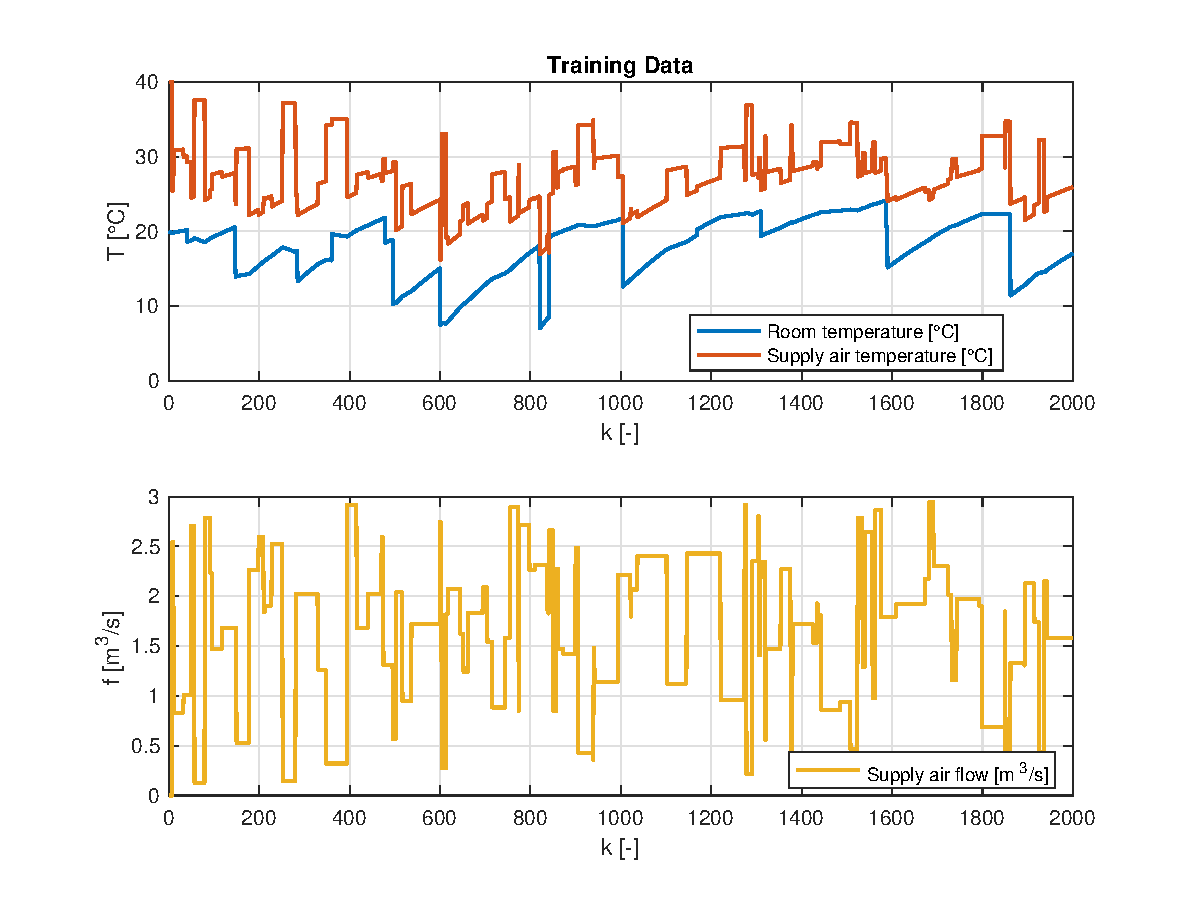
\includegraphics[width=0.95\columnwidth]{figures/training_data}
\caption{\label{fig:Q-Learning-training-data}Q-Learning training data consists
of $2,000$ data points ($\sim10$ hours) divided into $15$ continuous
time intervals during which the room was heated from a cold condition.
The room temperature $T_{z_{k}}\sim x_{k}$, supply air flow rate
$u_{k}$, and also supply air temperature $T_{s}$ calculated from
(\ref{eq:supply-air-temperature}) are shown. }
\end{figure}
Q function was calculated by the proposed method and optimal control
policy $\pi^{*}$ was found after several policy iterations (around
five suffice). Values $\gamma=0.999$ and $\xi=10^{-5}$ were used
in the algorithm. It is important that $u_{k}^{\pi}$ must excite
the process to cover the state-action space. The control actions must
be partly randomized to get a valid training dataset. This is related
to the well known problem of exploration-exploitation trade-off. Fig.
(\ref{fig:Q-Learning-with-Gaussian}) shows the trajectory of optimal
policy as a curve connecting the minima of Q function with respect
to $u$.

\begin{figure}
\centering{}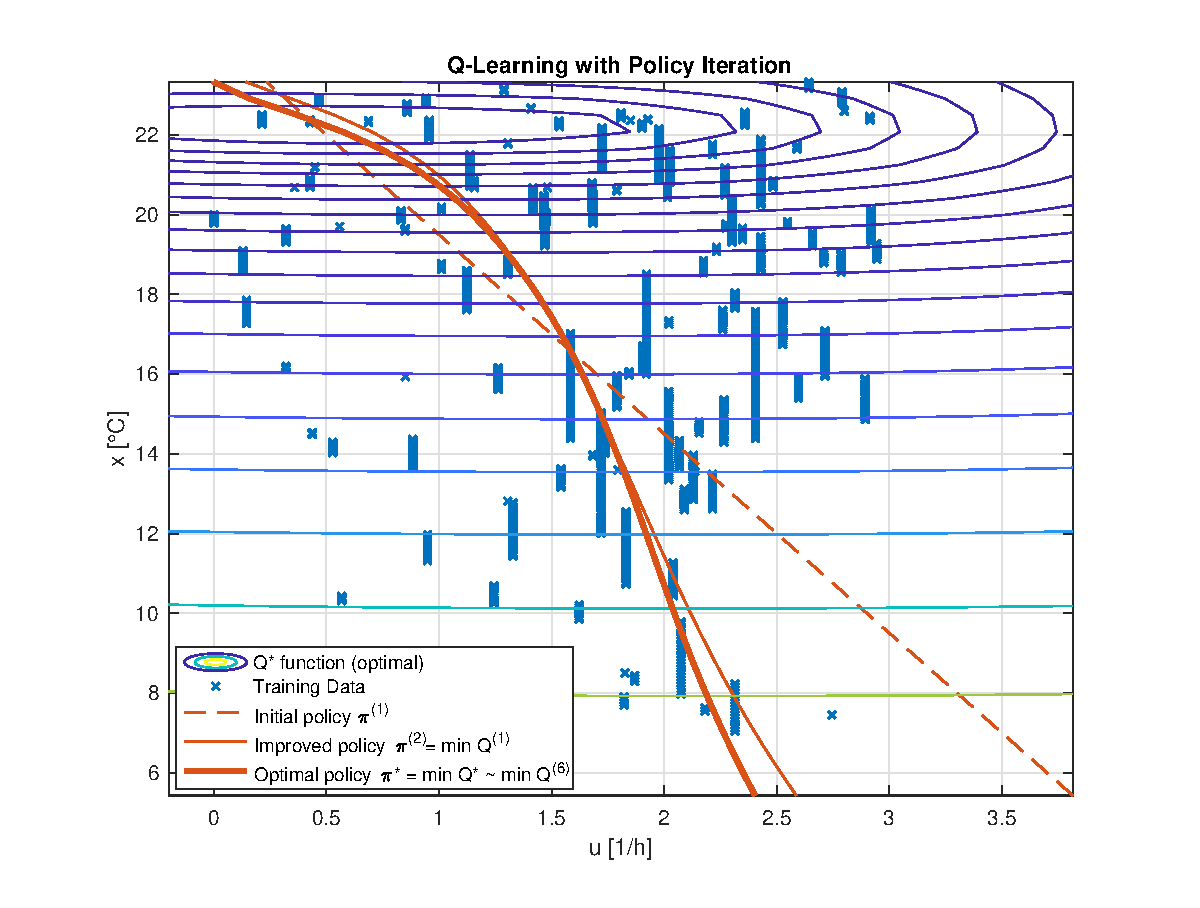
\includegraphics[width=0.95\columnwidth]{figures/q_learning_improved}
\caption{\label{fig:Q-Learning-with-Gaussian}Q-Learning with GPR and Policy
Iteration. $Q^{*}$ contours and policies $\pi^{(1)},\pi^{(2)}$ and
$\pi^{*}$ (highlighted) calculated from (\ref{eq:q-function-policy}).}
\end{figure}
This Q learning result makes good sense intuitively. The air exchange
rate $u_{k}$ equals the heat losses when the room temperature is
at the set point. Then it increases if the temperature is lower in
order to heat the interior. Therefore, there is a negative feedback
as expected. However, this feedback gain becomes smaller when the
control error is greater because the large air flows are less effective
for heating due to limited heat exchanger effectiveness and the decreasing
supply air temperature. Instead, the electrical fan noise and the
air flow would just annoy the occupants. Also, the fan would use more
electricity. All this is modeled by the second term in $\ell$. As
such, the policy resembles a proportional feedback controller with
variable gain. It does not have any integral action whereas a proportional
integral derivative (PID) controller would be normally used for similar
purpose. However, it can be shown that the integral action can be
added by augmenting the state space with temperature time difference
and considering the time difference $u_{k}-u_{k-1}$ as the control
action. Recall that the integral action is important in order to reject
unmeasured slow disturbances.

\subsection{Q-Learning Evaluation}

The results from Q-Learning were compared to multiple PI controllers
in terms of the cumulative loss function $L$ values. This function
represents the sum of all losses during an episode, i.e. $L=\sum_{k}\ell_{k}$.
An assuredly optimal value of cumulative loss $L^{*}$ is given by
the optimal policy $\pi^{*}$ from Q learning. A grid of proportional
and integral PI constants was considered so that it obviously contained
the optimal PI values (local minimum). All $L$ values were calculated
using (\ref{eq:loss-calculation}), starting at the same initial condition
$\mathrm{10^{o}C}$ over next 1,000 sampling periods considering $T_{sp}=22\unit{\lyxmathsym{\textdegree}C}$,
so the results are comparable. These values were compared in Fig.
(\ref{fig:Comparison-of-PI-Q-Learning}). The best PI controller parameters
from the grid were selected for Fig. (\ref{fig:Q-Learning-PI-PI}).
A PI controller designed for a linearized model of FCU at $u_{0}=1\left[\unitfrac{1}{h}\right],x_{0}=22\left[\unit{\lyxmathsym{\textdegree}C}\right]$
is also visualized. It can be observed that the best PI almost matches
the result of the Q learning whereas the model linearization based
result is different.

\begin{figure}
\centering{}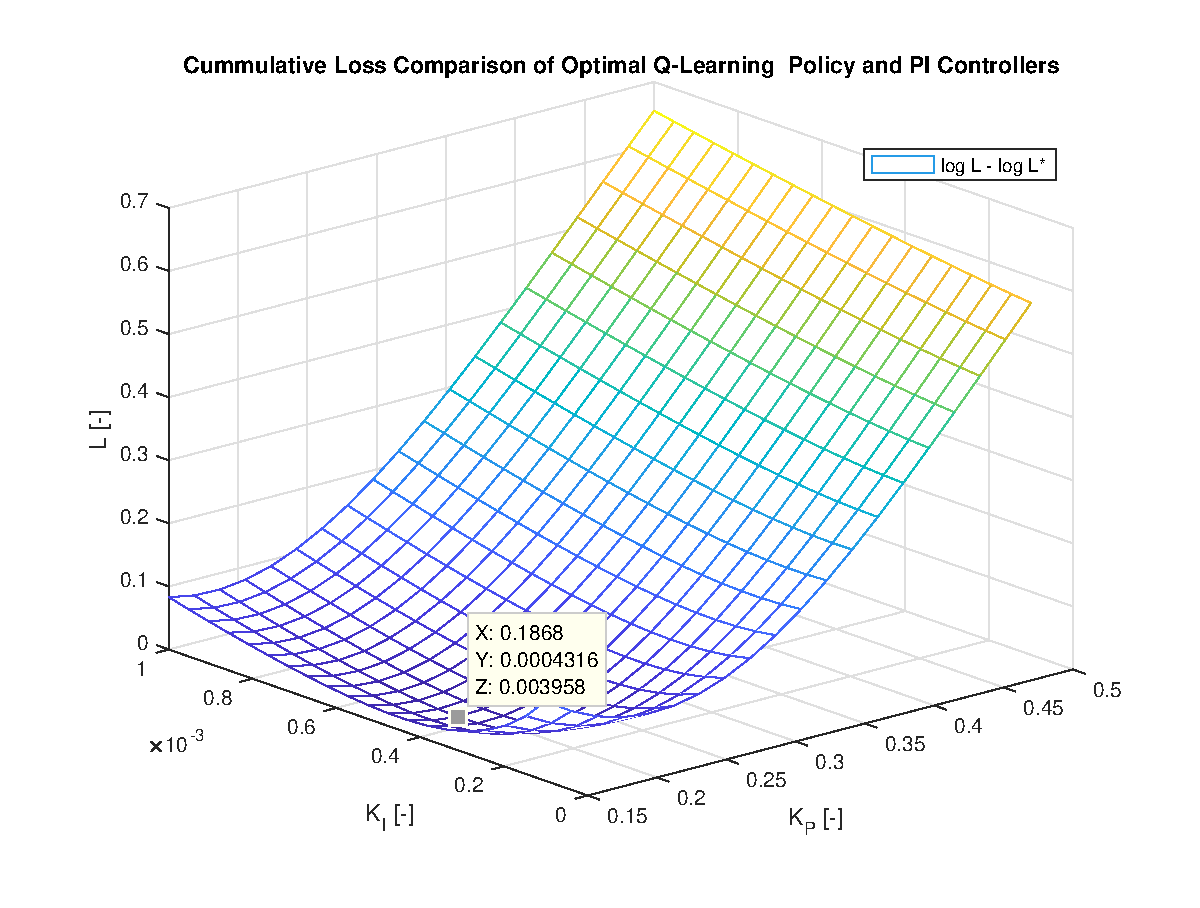
\includegraphics[width=0.95\columnwidth]{figures/q_learning_vs_pi_contr}
\caption{\label{fig:Comparison-of-PI-Q-Learning}Comparison of PI controllers
cumulative losses $L$ with optimal policy cumulative loss $L*$.}
\end{figure}
\begin{figure}
\centering{}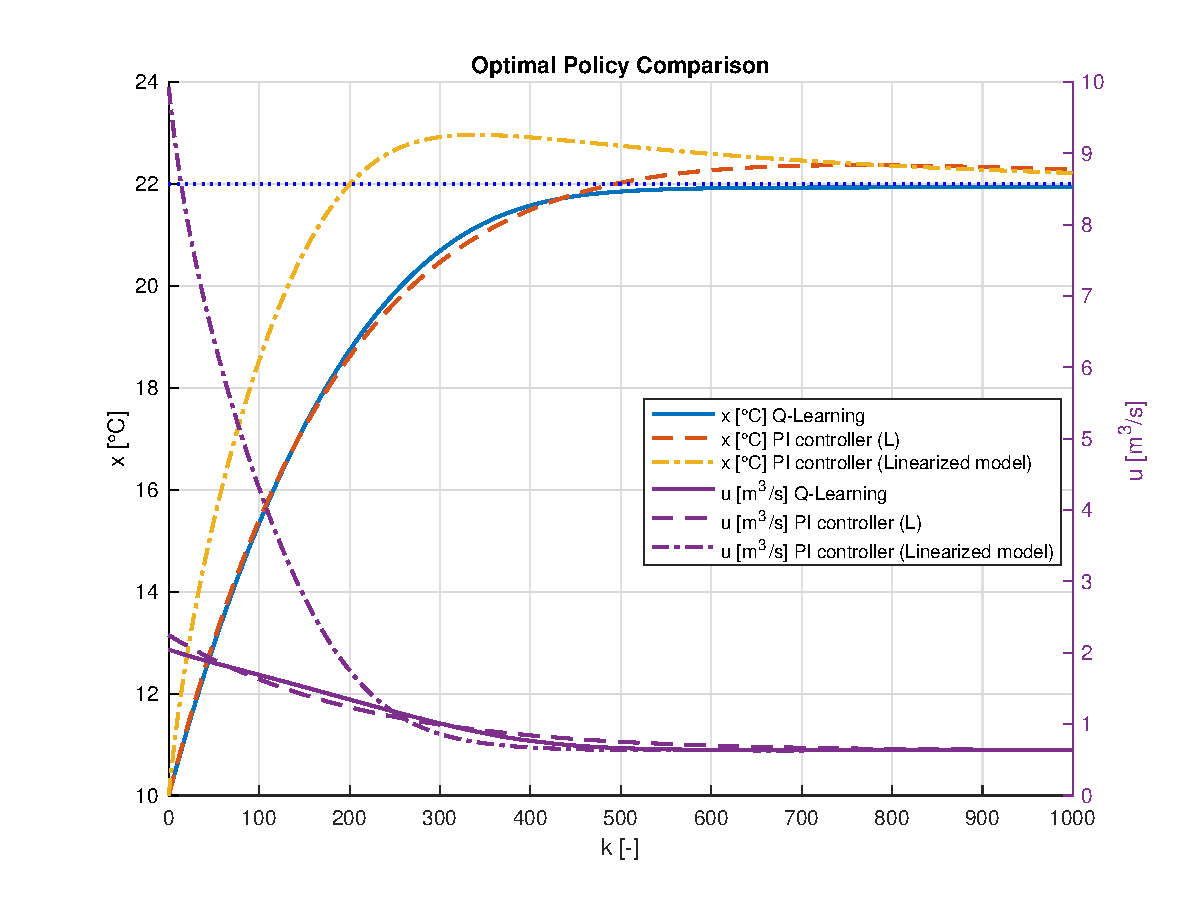
\includegraphics[width=0.95\columnwidth]{figures/optimal_policy}
\caption{\label{fig:Q-Learning-PI-PI}Comparison of Q-Learning optimal control
policy, PI controller designed by cumulative loss comparison and PI
controller designed from linearized model of FCU. The results are
presented on nonlinear FCU model.}
\end{figure}
Next, the controllers and the Q learning were tested considering the
net heat load/heat loss $q_{L}$ not constant but uniformly distributed
over $\left[-9,-5\right]$. The result is shown in Fig. (\ref{fig:Q-Learning-PI-PI-noisy}).
Note that Q-Learning designed controller is robust towards such a
noise. It should be noted that the same noise was used to generate
the learning data for this test, not only when simulating the controller.

\begin{figure}
\centering{}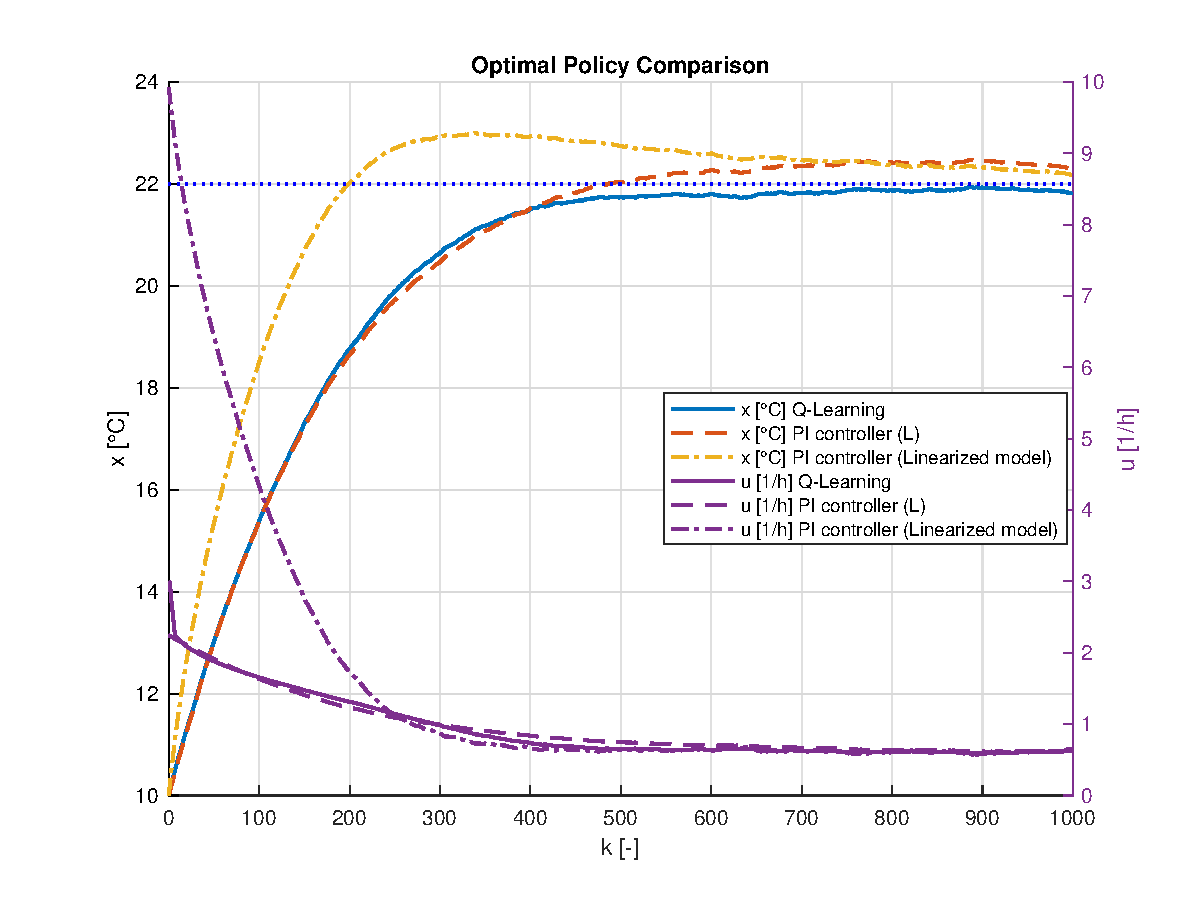
\includegraphics[width=0.95\columnwidth]{figures/optimal_policy_noisy}
\caption{\label{fig:Q-Learning-PI-PI-noisy}Comparison of Q-Learning optimal
control policy, PI controller designed by cumulative loss comparison
and PI controller designed from linearized model of FCU. The results
are presented on nonlinear FCU model with noisy net heat load/heat
loss $q_{L}$.}
\end{figure}

\section{CONCLUSIONS\label{sec:CONCLUSIONS}}

This paper described a practical approach of using GPR based Q-Learning
algorithm to find a control law for a completely unknown nonlinear
process based on a historical dataset of a medium size $\sim10^{3}$.
Engineers face such problem often and a solution is of practical interest.
An efficient GPR approach was used to calculate an unbiased Q function
value estimate in any point in the state-action space. The policy
iterations were used to optimize the controller. This method typically
converges rapidly. The optimal control law was then fully defined
by the minima of a GP. This represents a numerical optimization in
a low dimensional space of controller outputs and is thus numerically
trackable. Although not explained in this paper, GP can be globally
minimized even if it is not convex, see \cite{ecc19ref:Franey_Branch_and_Bound_Algo}.
An unbiased Q estimate makes the method insensitive to noise affecting
the process. Our approach is consistent with the Least-Squares Temporal
Difference Learning (LSTD) \cite{ecc19ref:Bratke_Linear_Least_Squares_Algo}
using GPR. The approach can be integrated with the GPR sparse form
in order to lower the dimensionality. However, details of this reduction
are currently a subject of research. The approach was verified on
a simple linear model against Q function calculated as a solution
of Riccati equation, this verification is not part of the paper. It
was then tested on a simplified nonlinear one-input one-state FCU
simulation model and an optimal control policy $\pi^{*}$ was calculated.
The result makes sense intuitively, the feedback gain is gradually
decreasing with the control error. A grid of PI controllers were compared
in terms of cumulative loss $L$ towards $L^{*}$,  found by the Q-learning.
The best PI controller from the grid was slightly worse than $L^{*}$.
However, such direct controller search is impractical without a simulation
model because it requires evaluating many controllers from defined
initial conditions and affected by defined disturbances. Also, a PI
controller was designed based on a linearized FCU model and PI tuning
rules. This traditional approach could actually be used in practice
together with, for example, Ziegler Nichols PID calibration method.
The controllers were compared in Section \ref{sec:RESULTS} and the
performance of PI designed using linearized FCU was shown to be worse
than both Q-Learning and the PI found by direct search. Here the problem
may be both linearization point and PID tuning rule which does not
minimize the loss (\ref{eq:loss-calculation}). Although the example
was a single input single output control problem, the method applies
to multidimensional problems without modifications. The whole process
was described for reader's understanding on the high level. Many technical
details were mentioned just briefly. However, the method is simple
and straightforward.

The main pitfalls of the process may be also pointed out. It is necessary
to choose a kernel function and several hyperparameters. However these
choices affect the accuracy, the method should still converges to
the same Q function asymptotically with growing dataset. The optimization
of hyperparameters in connection with the proposed approach is our
current research topic. Although result with only one kernel (SE times
quadratic) was presented, different kernels were also tried with similar
results, the hyperparameters were chosen reasonably and the kernels
were smooth. The method assumes the process state is measured without
error. This is not realistic in most control applications. The state
may be often approximated by measurements and lagged measurements
and control actions. Although the Q-learning seems to work well if
the approximation is reasonable, an optimal state approximation is
currently investigated in terms of dimension versus accuracy trade-off.
The training dataset must provide exploration and cannot be obtained
by running a fixed controller. A control action randomization is necessary.
A stabilizing initial controller is required. This does not seem to
be a serious constraint in many practical applications such as building
control. 

Overall, the method gives reasonably consistent results.

\bibliographystyle{plain}
\bibliography{ecc19ref}

\end{document}
